\documentclass{article}

\usepackage{packages}
\usepackage{environments}
\usepackage{commands}

\begin{document}

\title{Лекции по Численным методам}
\author{Лектор: Тараканов Александр}
\date{Весна 2024}

\maketitle
\tableofcontents

\ProvidesFile{lecture-02.tex}[Лекция 2]

\newpage

\section{Прямые методы решения систем линейных уравнений}

\subsection*{Постановка задачи}

Рассмотрим систему уравнений:

\begin{equation}\label{SLE}
    \begin{cases}
        A_{11}x_1 + \ldots A_{1n}x_n = y_1\\
        \ldots\\
        A_{n1}x_1 + \ldots + A_{nn}x_n = y_n
    \end{cases}
\end{equation}

Система уравнений \eqref{SLE} называется линейной системой уравнений (СЛУ). $A_{ij}$ --- матрица коэффициентов, $y_i$ --- правая часть и $x_i$ --- неизвестные

Про СЛУ естественно говорить на языке линейных пространств и операторов: пусть задан линеный оператор $A: X \longrightarrow Y$, вектор $y \in Y$ и требуется найти его прообраз $x \in X: Ax = y$

\subsection*{Предположения}

В общем случае при решении СЛУ возможны несколько случаев:

\begin{itemize}
    \item Решение существует и единственно $\ker A = 0$ и $y \in \Im A$

    \item Решение существует, но не единственно $\ker A \neq 0$ и $y \in \Im A$

    \item Решения не существует $y \notin \Im A$
\end{itemize}

В данном курсе мы будем рассматривать только частный случай: $\ker A = 0$ и $\Im A = Y$ или $\mathrm{coker} \, A = 0$

Иными словами: будем считать, что $X$ и $Y$ --- линейные пространства одинаковой размерности $n$, матрица СЛУ $A$ является несингулярной (квадратной и невырожденной)

В такой постановке задача $Ax=y$ определена корректно и решение существует и единственно для любой правой части

Далее в курсе будут разбираться различные алгоритмы поиска решения в зависимости от свойств матрицы $A$

\subsection{Нижние и верхние треугольные матрицы}

\begin{definition}
Матрица $L$ называется \textit{нижней треугольной} матрицей, если $L_{ij} = 0$, если $j > i$
\end{definition}

\begin{definition}
Матрица $U$ называется \textit{верхней треугольной} матрицей, если $U_{ij} = 0$, если $j < i$
\end{definition}

Нижние и верхние треугольные матрицы обладают следующим важным свойством

\begin{claim}
Пусть $A$ и $B$ нижние (верхние) треугольные матрицы, то и матрица $C = AB$ является нижней (верхней) треугольной матрицей
\end{claim}

\begin{proof}
    Для доказательства вычислим значение матричного элемента $C_{ij}$ при $j > i$ для нижних треугольных матриц:

    \[
    C_{ij} = \sum\limits_{k = 1}^n A_{ik} \cdot B_{kj} = \sum\limits_{k = 1}^i A_{ik} \cdot B_{kj} + \sum\limits_{k = i+1}^n A_{ik} \cdot B_{kj} = \sum\limits_{k = 1}^i A_{ik} \cdot 0 + \sum\limits_{k = i+1}^n 0 \cdot B_{kj} = 0
    \]
\end{proof}

\subsubsection*{Решение системы с нижней треугольной матрицей}

Рассмотрим СЛУ с нижней треугольной матрицей $L$:

\begin{equation*}\label{lowerTrigSLE}
    \begin{cases}
        L_{11}x_1 &= y_1\\
        L_{21}x_1 + L_{22}x_2 &=y_2\\
        \ldots\\
        L_{n1}x_1 + \ldots + L_{nn}x_n &= y_n
    \end{cases}
\end{equation*}

Тогда решение можно найти, исключая неизвестные:

\begin{equation*}
\begin{aligned}
    &x_1 = y_1 / L_{11}\\
    &x_2 = (y_2 - L_{21}x_1) / L_{22}\\
    &\ldots\\
    &x_i = \left(y_i - \sum\limits_{j = 1}^{i - 1} L_{ij}x_j\right) / L_{ii}\\
    &\ldots
\end{aligned}
\end{equation*}

\subsubsection*{Решение системы с верхней треугольной матрицей}

Рассмотрим СЛУ с верхней треугольной матрицей $U$:

\begin{equation*}\label{upperTrigSLE}
    \begin{cases}
        U_{11}x_1 + \ldots + U_{1n}x_n &= y_1\\
        \ldots\\
        U_{(n-1)(n-1)}x_{n-1} + \ldots + U_{(n-1)n}x_{n} &= y_{n-1}\\
        U_{nn}x_1 &= y_n
    \end{cases}
\end{equation*}


Тогда решение можно найти, исключая неизвестные:

\begin{equation*}
\begin{aligned}
    &x_n = y_n / U_{nn}\\
    &x_{n-1} = (y_{n-1} - U_{(n-1)n}x_{n-1}) / U_{(n-1)(n-1)}\\
    &\ldots\\
    &x_i = \left(y_i - \sum\limits_{j = i+1}^n U_{ij}x_j\right) / U_{ii}\\
    &\ldots
\end{aligned}
\end{equation*}

\subsection{Решение системы уравнений с помощью LU разложения}

Пусть есть СЛУ $Ax = y$

Идея алгоритма состоит в следующем:

\begin{itemize}
    \item Представить матрицу $A$ в виде произведения: $A = LU$, где $L$ --- нижняя треугольная матрица, $U$ --- верхняя треугольная
    \item Решить систему $Lz = y$
    \item Решиить систему $Ux = z$
\end{itemize}

\begin{proof}
    Пусть $x$ --- решение исходной системы. Тогда

    \[
    Ax = LUx = L(Ux) = Lz = y
    \]
\end{proof}

\paragraph{Замечание}

\begin{itemize}
    \item В общем случае LU разложение не определено однозначно: если $D$ --- невырожденная диагональная матрица, то можно построить другое LU разложение по уже имеющемуся:

    \[
    A = LU = LDD^{-1}U = (LD)(D^{-1}U) = L'U'
    \]

    Данную неопределенность можно решить, зафиксировав, что $L_{ii} = 1$ или $U_{ii} = 1$
\end{itemize}

\subsubsection*{Алгоритм построения LU разложения}

Рассмотрим случай, когда диагональ верхней треугольной матрицы $U_{ii} = 1$. Будем вычислять элементы матриц $L$ и $U$ построчно:

\begin{itemize}
    \item Первая строка: $L_{11}U_{11} = A_{11}$ и $U_{11} = 1$, поэтому $L_{11} = A_{11} / U_{11}$ (перемножили 1-ую строку и 1-ый столбец). Далее вычислим $U_{1i}$: (перемножаем 1-ую строку и $i$-ый столбец)

    \[
    L_{11}U_{1i} = A_{1i} \iff U_{1i} = A_{1i} / L_{11}
    \]

    \item Вторая строка: $L_{21}U_{11} = A_{21}$ и $U_{11} = 1$, поэтому $L_{21} = A_{21} / U_{11}$ (перемножили 1-ую строку и 2-ый столбец). Далее вычислим $L_{22}$: (перемножим 2-ую строку и 2-ый столбец)

    \[
    L_{21}U_{12} + L_{22}U_{22} = A_{22} \iff L_{22} = (A_{22} - L_{21}U_{12}) / U_{22}
    \]

    Теперь вычислим $U_{2i}$: (перемножим 2-ую строку и $i$-ый столбец)

    \[
    L_{21}U_{12} + L_{22}U_{2i} = A_{2i} \iff U_{2i} = (A_{2i} - L_{21}U_{12}) / L_{22}
    \]

    И так далее

    \item В итоге получаем, что вычислить $i$-ую строку матрицы $L$, можно следующим образом: $(j \leqslant i)$

    \[
    L_{ij} = \left(A_{ij} - \sum\limits_{k = 1}^{j - 1} L_{ik}U_{kj}\right) / U_{jj}
    \]

    А $i$-ая строка матрицы $U$ вычисляется так: $(j > i)$

    \[
    U_{ij} = \left(A_{ij} - \sum\limits_{k = 1}^{i-1}L_{ik}U_{kj}\right) / L_{ii}
    \]
\end{itemize}

\paragraph{Замечание}

Если мы задаем диагональные элементы нижней треугольной матрицы $L$, то задача сводится к уже решенной:

\[
A^{\top} = L'U' \iff A = (U')^{\top} (L')^{\top} = LU
\]

Данный алгоритм позволяет найти LU разложение для матрицы $A$ единственным образом, если зафиксировать диагональные элементы матрицы $U$ или $L$. Однако если на $m$-ом шаге окажется, что $L_{mm} = 0$, то алгоритм позволяет найти только лишь LU разложение главного минора порядка $m$ матрицы $A$:

\[[A]_m = [L]_m [U]_m,\]

где $[L]_m$ и $[U]_m$ --- нижняя и верхняя треугольные матрицы, вычисленные за $m$ шагов

В общем случае, данный алгоритм не гарантирует сходимости к LU разложению для матрицы $A$, однако существует класс матриц $A$, для которых алгоритм корректно находит LU разложение

\subsubsection*{Класс матриц}

Необходимо проверить, есть ли нули на диагонали матрицы $L$, тогда вышеописанный алгоритм будет работать корректно

\begin{claim}
    Если $\forall \, m \in \{1, \ldots n\}: \det [A]_m \neq 0$, то $L_{mm} \neq 0$
\end{claim}

\begin{proof}
    Докажем от противного. Зафиксируем $m \in \{1, \ldots, n\}$ и $\det [A]_m \neq 0$. Пусть $L_{ii} \neq 0$ при $i < m$ и $L_{mm} = 0$. Тогда верно, что

    \[
    [A]_m = [L]_m [U]_m \implies \det [A]_m = \det [L]_m \cdot \det [U]_m = \prod\limits_{i = 1}^m L_{ii} \cdot \prod\limits_{i = 1}^m U_{ii} = 0
    \]

    Получили противоречие, что определитель главного минора $[A]_m$ не равен $0$
\end{proof}

В общем случае данное утверждение сложно проверить. Если матрица является симметричной положительно определенной (SPD), то тогда оно выполнено по \href{https://en.wikipedia.org/wiki/Sylvester%27s_criterion}{критерию Сильвестра}

Помимо SPD матриц, часто встречаются матрицы со следующим особым свойством

\begin{definition}
    Матрица $A$ называется \textit{матрицей с диагональным преобладанием}, если $\forall \, i \in \{1, \ldots, n\}$

    \[
    |A_{ii}| - \sum\limits_{j \neq i} |A_{ij}| > 0
    \]
\end{definition}

Видно, что главный минор такой матрицы также является матрицей с диагональным преобладанием. Докажем следующее утверждение

\begin{claim}
    Матрица с диагональным преобладанием является несингулярной
\end{claim}

\begin{proof}
    Докажем от противного. Пусть матрица вырожденная. Тогда $\exists \, x \in \mathbb{R}^n: Ax = 0$. Найдем максимальный по модулю элемент в векторе $x: |x_i| = \max\limits_{j} |x_j|$ и рассмотрим $i$-ую строку $Ax$:

    \[
    0 = \left|\sum\limits_{j} A_{ij}x_j\right| = |x_i| \cdot \left|\sum\limits_{j} A_{ij} \frac{x_j}{|x_i|}\right| =
    %
    |x_i| \cdot \left|A_{ii} + \sum\limits_{j \neq i} A_{ij} \cdot \frac{x_j}{|x_i|}\right| \geqslant |x_i| \cdot \left|A_{ii} - \sum\limits_{j \neq i} |A_{ij}| \cdot \frac{|x_j|}{|x_i|}\right| > 0
    \]

    Предпоследнее неравенство верно по обратному неравенства треугольника. Последнее неравенство верно, так как матрица $A$ является матрицей с диагональным преобладанием, а отношение $|x_j| / |x_i| < 1$ при $j \neq i$.

    Получили противоречие
\end{proof}


\subsection{Решение системы уравнений с помощью разложения Холецкого}

Пусть есть СЛУ $Ax = y$ и матрица $A$ является SPD матрицей. Тогда существует специальный вид (причем единственный) LU разложения --- разложение Холецкого:

\[A = LL^{\top},\]

где $L$ --- нижняя треугольная матрица с положительными элементами на диагонали

\begin{claim}
    Существование разложения Холецкого
\end{claim}

\begin{proof}
    Пусть задано какое-то LU разложение: $A = LU$ (существование его доказывалось ранее). Тогда верно следующее:

    \[
    LU = A = A^{\top} = U^{\top} L^{\top}
    \]

    Домножим слева равенство на $L^{-1}$:

    \[
    U = L^{-1} U^{\top} L^{\top}
    \]

    Теперь домножим справа равенство на $(L^{\top})^{-1}$:

    \[
    U (L^{\top})^{-1} = L^{-1} U^{\top} = D
    \]

    Получим, что слева у нас верхняя треугольная матрица, а справа нижняя треугольная матрица, поэтому и справа, и слева диагональная матрица $D$

    Рассмотрим исходное LU разложение:

    \[
    A = LU = L \cdot (D L^{\top}) = L D^{1/2} D^{1/2} L^{\top} = (L D^{1/2}) (L D^{1/2})^{\top} = L' L'^{\top}
    \]

    Причем диагональные элементы $D$ могут быть только положительными, так как $A$ является SPD матрицей и $L$ --- матрица перехода от одного базиса к другому

\end{proof}

\begin{claim}
    Единственность разложения Холецкого
\end{claim}

\begin{proof}
    Единственность доказывается вместе с построением алгоритма вычисления, аналогичному для LU разложения

    \begin{itemize}
        \item $L_{11}L_{11} = A_{11} \iff L_{11} = \sqrt{A_{11}}$

        \item $i$-ая строка при $j < i$:

        \[
        \sum\limits_{k = 1}^{j - 1} L_{ik} L_{kj} + L_{ij}L_{jj} = A_{ij} \iff L_{ij} = \left(A_{ij} - \sum\limits_{k = 1}^{j - 1} L_{ik} L_{kj}\right) / L_{jj}
        \]

        \item Диагональные элементы $L_{ii}$:

        \[
        L_{ii} = \sqrt{A_{ii} - \sum\limits_{k = 1}^{j - 1} L_{ik} L_{kj}}
        \]
    \end{itemize}
\end{proof}

\subsection{Решение систем уравнений с помощью алгоритма Гаусса}

Пусть есть СЛУ $Ax = y$

Будем решать ее алгоритмом Гаусса: сначала применять прямой алгоритм
Гаусса, потом обратный. Данный алгоритм является одним из способов построения LU разложения

Во время прямого алгоритма Гаусса мы будем приводить матрицу $A$ к ступенчатому виду, выполняя операции над строками:

\begin{itemize}
    \item 1 тип: $i \mapsto i \cdot \lambda, \lambda \neq 0$
    \item 2 тип: $i \leftrightarrow j$
    \item 3 тип: $i \mapsto i + j \cdot \lambda$
\end{itemize}


Во время обратного хода мы теми же действиями будем приводить матрицу $A$ к улучшенному ступенчатому виду, чтобы главные коэффициенты были равны $1$

Каждой операции над строками однозначно сопоставляется умножение слева на матрицу

Сложность алгоритма Гаусса составляет $O(n^3)$, где $n$ --- разномерность матрицы $A$. Поэтому данные алгоритмы не используются для решения СЛУ больших размерностей

\ProvidesFile{lecture-03.tex}[Лекция 3]

\newpage

\section{Норма и анализ сходимости}

\begin{definition}
    Пусть задано линейное векторное пространство $V$ над полем $\mathbb{R}$. \\ Функцию $\lVert \cdot \rVert: V \longrightarrow \mathbb{R}$ будем называть \textit{нормой}, если выполнены следующие свойства:

    \begin{itemize}
        \item $\forall \, x \in V: \lVert x \rVert \geqslant 0$
        \item $\lVert x \rVert = 0 \iff x = 0$
        \item $\lVert \alpha x \rVert = |\alpha| \cdot \lVert x \rVert$
        \item $\forall \, x, y \in V: \lVert x + y \rVert \leqslant \lVert x \rVert + \lVert y \rVert$ --- неравенство треугольника
    \end{itemize}

    Пространство $V$ с нормой $\lVert \cdot \rVert$ называется \textit{нормированным пространством}
\end{definition}

\subsection{Векторные $l_p$ нормы}

Важным примером норм является $l_p$ норма. Пусть $V = \mathbb{R}^n$. Тогда для $x \in V$, который будем записывать в виде вектор-столбца $x = [x_1, \ldots, x_n]^{\top}$, определим $l_p$ норму:

\[
\lVert x \rVert_p = \left(\sum\limits_{i = 1}^n |x_i|^p\right)^{1/p}
\]

Существуют особые виды $l_p$ нормы:

\begin{itemize}
    \item $p = 1: \lVert x \rVert_1 = |x_1| + \ldots + |x_n|$
    \item $p = 2: \lVert x \rVert_2 = \sqrt{|x_1|^2 + \ldots + |x_n|^2}$
    \item $p = \infty: \lVert x \rVert_{\infty} = \max\limits_{i} |x_i|$
\end{itemize}

\begin{claim}
    Докажем, что приведенные функции являются нормами
\end{claim}

\begin{proof}
    Разберем каждый случай по отдельности:

    \begin{enumerate}
        \item Случай $p = 1$

            \begin{itemize}
                \item $\lVert x \rVert_1 \geqslant 0$ очевидно. Пусть $\lVert x \rVert = 0$. Тогда $|x_1| + \ldots + |x_n| = 0 \iff x_1 = \ldots = x_n = 0 \iff x = 0$. \\В обратную сторону очевидно

                \item $\lVert \alpha x \rVert_1 = |\alpha x_1| + \ldots + |\alpha x_n| = |\alpha| \cdot (|x_1| + \ldots + |x_n|) = |\alpha| \cdot \lVert x \rVert_1$

                \item Зафиксируем $x, y \in V$. Тогда
                \[
                \lVert x + y \rVert_1 = \sum\limits_{i = 1}^n |x_i + y_i| \leqslant \sum\limits_{i = 1}^n |x_i| + \sum\limits_{i = 1}^n |y_i| = \lVert x \rVert_1 + \lVert y \rVert_1
                \]
            \end{itemize}

        \item Случай $p = 2$

            \begin{itemize}
                \item Первые три свойства проверяются аналогично. Докажем только неравенство треугольника. Зафиксируем $x, y \in V$ и воспользуемся \href{https://en.wikipedia.org/wiki/Cauchy%E2%80%93Schwarz_inequality}{неравенством Коши-Буняковского}:

                \[
                \lVert x + y \rVert_2^2 = \sum\limits_{i = 1}^n |x_i + y_i|^2 = \sum\limits_{i = 1}^n |x_i|^2 + \sum\limits_{i = 1}^n |y_i|^2 + 2 \sum\limits_{i = 1}^{n} |x_i| \cdot |y_i|
                \leqslant
                %
                \lVert x \rVert_2^2 + \lVert y \rVert_2^2 + 2 \lVert x \rVert_2 \cdot \lVert y \rVert_2 = (\lVert x \rVert_2 + \lVert y \rVert_2)^2
                \]
            \end{itemize}

        \item Случай $p \in \mathbb{R}: p > 1$

            \begin{itemize}
                \item Первые три свойства проверяются аналогично. Докажем неравенство треугольника

                \item Предположим, что $x, y \in V: x \neq 0, y \neq 0$ и $\forall \, i \in \{1, \ldots, n\}: x_i \geqslant 0$ без ограничения общности рассуждений. \\ Зафиксируем $x$ и будем искать максимум $f(y) = \lVert x + y \rVert_p$ по $y$ при условии, что $\lVert y \rVert_p = C = \mathrm{const}$

                Из курса математического анализа известно, что непрерывная функция на компакте достигает своего максимума. Пусть $f(y)$ достигает максимума в точке $y^{\star}$

                Тогда запишем уравнение касательной плоскости к поверхности $\lVert y \rVert_p = C$: \\($dy = [dy_1, \ldots, dy_n]^{\top}$ --- вектор приращений)

                \begin{equation}\label{tangent_plane}
                \sum\limits_{i = 1}^n \frac{\partial}{\partial y_i} \lVert y \rVert_p^p \, dy_i = \sum\limits_{i = 1}^n p |y_i|^{p - 1} \, dy_i = 0 = \Big\langle \nabla \lVert y \rVert_p^p, \, dy \Big\rangle
                \end{equation}

                \item Так как $y^{\star}$ --- точка экстремума функции, то найдем производную $f(y)^p$:

                \begin{equation}\label{max_point}
                \frac{d}{dy}f(y^{\star})^p = \sum\limits_{i = 1}^{n} p |x_i + y^{\star}|^{p - 1} \, dy_i = 0 = \Big\langle \nabla f(y^{\star})^p, \, dy \Big\rangle
                \end{equation}

                \item Из \eqref{tangent_plane} в точке $y^{\star}$ и \eqref{max_point} следует, что векторы

                \[\nabla \lVert y^{\star} \rVert_p^p = \Big[|y^{\star}_1|^{p-1}, \ldots, |y^{\star}_n|^{p-1}\Big]^{\top}
                \]
                и
                \[\nabla f(y^{\star})^p = \Big[|x_1 + y^{\star}_1|^{p-1}, \ldots, |x_n + y^{\star}_n|^{p-1}\Big]^{\top}
                \]

                перпендикулярны вектору приращений $dy$, а значит коллинеарны:

                \[
                |x_i + y^{\star}_i| = \lambda |y^{\star}_i|
                \]

                \item Так как $y^{\star}$ --- точка максимума, то в знаки $x_i$ и $y^{\star}_i$ должны совпадать. То есть $y_i = k x_i$ для некоторого $k > 0$, которое можно найти следующим образом:

                \[
                k = \frac{\lVert y \rVert_p}{\lVert x \rVert_p} = \frac{C}{\lVert x \rVert_p}
                \]

                \[
                \lVert x + y \rVert_p \leqslant \lVert x + y^{\star} \rVert_p = \lVert x + kx \rVert_p = \lVert x \rVert_p + \lVert kx \rVert_p = \lVert x \rVert_p + \lVert y \rVert_p
                \]

            \end{itemize}

        \item Случай $p = \infty$

            \begin{itemize}
                \item Рассмотрим следующий предел:

                \[
                \lim\limits_{p \to \infty} \lVert x \rVert_p
                \]

                \item Пусть дан вектор $x \in V: \lVert x \rVert_{\infty} = |x_k|$. Тогда

                \[
                \lVert x \rVert_{\infty} = |x_k| = \left(\sum\limits_{i = 1}^n |x_i|^p\right)^{1/p} \leqslant \lVert x \rVert_p \leqslant \left(\sum\limits_{i = 1}^n |x_k|^p\right)^{1/p} = n^{1/p} \lVert x \rVert_{\infty} = n^{1/p} |x_k|
                \]

                \item Отсюда и из $n^{1/p} \longrightarrow 1$ при $p \longrightarrow \infty$ видно, что $\lVert x \rVert_{\infty} = \lim\limits_{p \to \infty} \lVert x \rVert_p$

                \item Теперь мы можем доказать, что $\lVert x \rVert_{\infty}$ является нормой по предельным переходам
            \end{itemize}
    \end{enumerate}
\end{proof}

\begin{definition}
    Пусть задано линейное векторное пространство $V$ над полем $\mathbb{R}$. \\ Функцию $\rho: V \times V \longrightarrow \mathbb{R}$ будем называть \textit{метрикой}, если выполнены следующие свойства:

    \begin{itemize}
        \item $\forall \, x, y \in V: \rho(x, y) \geqslant 0$
        \item $\rho(x, y) = 0 \iff x = y$
        \item $\forall \, x, y \in V: \rho(x, y) = \rho(y, x)$
        \item $\forall \, x, y, z \in V: \rho(x + z) \leqslant \rho(x, y) + \rho(y, z)$  --- неравенство треугольника
    \end{itemize}

    Пространство $V$ с метрикой $\rho$ называется \textit{метрическим пространством}
\end{definition}

Заметим, что любая норма на линейном пространстве задает метрику:

\[
\rho(x, y) = \lVert x - y \rVert
\]

\subsection{Сходимость по норме}

\begin{definition}
    Две нормы $\lVert \cdot \rVert_a$ и $\lVert \cdot \rVert_b$ (необязательно $l_p$ нормы) на нормированном пространстве $V$ называются эквивалентными, если $\exists \, C_1, C_2 > 0: \forall \, x \in V$

    \[
    C_1 \cdot \lVert x \rVert_a \leqslant \lVert x \rVert_b \leqslant C_2 \cdot \lVert x \rVert_b
    \]
\end{definition}

Известно, что на конечномерных пространствах все нормы являются эквивалентными. Будем говорить, что последовательность векторов $\{x_k\}$ сходится к $x$ по норме, если $\lVert x_k - x \rVert \longrightarrow 0$ при $k \longrightarrow \infty$. Так как все нормы являются эквивалентными, то для исследования сходимости можно использовать любую норму. Также для конечномерных пространств верно, что из покоордиантной сходимости следует сходимость по норме и наоборот

\subsection{Норма линейного оператора}

\begin{definition}
    Пусть задано нормированное пространство $V$ с нормой $\lVert x \rVert$. Пусть задан линейный оператор $A: V \longrightarrow V$. Определим норму линейного оператора следующим образом:

    \[
    \lVert A \rVert = \sup\limits_{\lVert x \rVert \neq 0} \frac{\lVert Ax \rVert}{\lVert x \rVert}
    \]
\end{definition}

\begin{claim}
    Докажем, что это действительно норма, и перечислим свойства
\end{claim}

\begin{itemize}
    \item Первые три свойства нормы выполняются
    \item Проверим неравенство треугольника:

    \[
    \lVert A + B \rVert = \sup\limits_{\lVert x \rVert \neq 0} \frac{\lVert Ax + Bx \rVert}{\lVert x \rVert} \leqslant
    %
    \sup\limits_{\lVert x \rVert \neq 0} \left(
    \frac{\lVert Ax \rVert}{\lVert x \rVert}
    +
    \frac{\lVert Bx \rVert}{\lVert x \rVert}
    \right) \leqslant
    %
    \sup\limits_{\lVert x \rVert \neq 0} \frac{\lVert Ax \rVert}{\lVert x \rVert}
    +
    \sup\limits_{\lVert x \rVert \neq 0} \frac{\lVert Bx \rVert}{\lVert x \rVert} = \lVert A \rVert + \lVert B \rVert
    \]

    \item Видно из определения нормы, что

    \[
    \lVert Ax \rVert \leqslant \lVert A \rVert \cdot \lVert x \rVert
    \]

    \item Оценим сверху норму композиции операторов $BA$:

    \[
    \lVert BAx \rVert = \lVert B (Ax) \rVert \leqslant \lVert B \rVert \cdot \lVert Ax \rVert \leqslant \lVert B \rVert \cdot \lVert A \rVert \cdot \lVert x \rVert
    \]

    Поэтому $\lVert BA \rVert \leqslant \lVert B \rVert \cdot \lVert A \rVert$

    \item Из линейности оператора следует, что

    \[
    \sup\limits_{\lVert x \rVert \neq 0} \frac{\lVert Ax \rVert}{\lVert x \rVert} = \sup\limits_{\lVert x \rVert \neq 0} \left\lVert A \cdot \left(\frac{x}{\lVert x \rVert}\right)\right\rVert = \sup\limits_{\lVert x \rVert = 1} \lVert Ax \rVert
    \]

    По этой причине норма любого линейного оператора на конечномерном линейном пространстве с $l_p$ нормой существует и конечна
\end{itemize}

\paragraph{Примеры}

\begin{itemize}
    \item Норма диагонального оператора $D_{n \times n} = D$ с помощью $l_p$ нормы:

    \[
    \sup\limits_{\lVert x \rVert = 1} \lVert Dx \rVert_p = \left(\sum\limits_{i = 1}^n |D_{ii}|^p \cdot |x_i|^p\right)^{1/p}
    \]

    Пусть $D_{kk} = \max\limits_{i} |D_{ii}|$. Тогда

    \[
    \left(\sum\limits_{i = 1}^n |D_{ii}|^p \cdot |x_i|^p\right)^{1/p} \leqslant \left(\sum\limits_{i = 1}^n |D_{kk}|^p \cdot |x_i|^p\right)^{1/p} = |D_{kk}| \left(\sum\limits_{i = 1}^n |x_i|\right)^{1/p}
    \]

    Получается, что

    \[
    \sup\limits_{\lVert x \rVert = 1} \lVert Dx \rVert_p \leqslant \max\limits_{i} |D_{ii}|
    \]

    Пример, на котором достигается максимум легко построить: возьмем $x = [0, \ldots, 1, \ldots, 0]^{\top}$ --- ненулевая координата только на $k$-ой позиции

    \item Рассмотрим $l_2$ норму на конечномерном линейном пространстве $V$. Пусть есть некоторый оператор $A$. Известно, что любой оператор можно разложить в виде композиции поворотов, отражений и растяжений вдоль осей с положительными коэффициентами --- \href{https://en.wikipedia.org/wiki/Singular_value_decomposition}{SVD}:

    \[
    A = U_1 D U_2,
    \]

    где $U_1, U_2$ --- ортогональные матрицы, которые сохраняют расстояние $\lVert U_1 x \rVert = \lVert U_2 x \rVert = \lVert x \rVert$

    \[
    \lVert A \rVert = \sup\limits_{\lVert x \rVert = 1} \lVert A x \rVert = \sup\limits_{\lVert x \rVert = 1} \lVert U_1 D U_2 x \rVert =  \sup\limits_{\lVert x \rVert = 1} \lVert D U_2 x \rVert =  \sup\limits_{\lVert x \rVert = 1} \lVert D x \rVert = \max\limits_{i} D_{ii}
    \]

    \item Рассмотрим $l_2$ норму на конечномерном линейном пространстве $V$. Пусть есть некоторый самосопряженный оператор $A$ (заданный SPD матрицей). Тогда представим его в следующем виде:

    \[
    A = U D U^{\top},
    \]

    где $U$ --- ортогональная матрица, $D$ --- диагональная матрица из собственный значений $\lambda_i$. Аналогично предыдущему пункту:

    \[
    \lVert A \rVert = \max\limits_{i} \lambda_i
    \]

    \item Рассмотрим $l_{\infty}$ норму на конечномерном линейном пространстве $V$ и произвольный оператор $A$

    \[
    \lVert A \rVert = \sup\limits_{\lVert x \rVert = 1} \lVert Ax \rVert_{\infty} = \max\limits_{i} \left|\sum\limits_j A_{ij} x_j\right| = \left| \sum\limits_j A_{kj} x_j \right|
    \]

    Заметим, что $A_{kj}$ и $x_j$ должны быть одного знака, иначе можно поменять знак координаты $j$ вектора $x$ на противоположный и значение увеличится, что противоречит максимальности выражения. Так как $\lVert x \rVert_{\infty} = 1$, тогда есть координата $|x_m| = 1$. Тогда заменим все $x_j$ на $1$, от этого норма не изменится. В итоге получили, что

    \[
    \lVert A \rVert = \max\limits_{i} \left|\sum\limits_j A_{ij}\right|
    \]
\end{itemize}

\subsection{Число обусловленности}

\begin{definition}
    Пусть на нормированном конечномерном пространстве $V$ задан невырожденный линейный оператор $A: V \longrightarrow V$. \textit{Числом обусловленности} линейного оператора будем называть следующее выражение:

    \[
    \kappa(A) = \lVert A \rVert \cdot \lVert A^{-1} \rVert
    \]
    %
    \\Видно, что $\kappa(A) = \kappa(A^{-1})$
\end{definition}

\begin{claim}
    Число обусловленности $\kappa(A) \geqslant 1$
\end{claim}

\begin{proof}
    \[
    \lVert x \rVert = \lVert A^{-1}Ax \rVert \leqslant \lVert A^{-1} \rVert \cdot \lVert Ax \rVert \leqslant \lVert A^{-1} \rVert \cdot \lVert A \rVert \cdot \lVert x \rVert = \kappa(A) \cdot \lVert x \rVert
    \]
\end{proof}

\begin{claim}
    Пусть $A$ --- самосопряженный линейный оператор и задана $l_2$ норма. Тогда число обусловленности равно

    \[
    \kappa(A) = \frac{\max_{i} \lambda_i}{\min_{i} \lambda_i},
    \]
    где $\lambda_i$ --- собственное значение матрицы $A$
\end{claim}

\begin{proof}
    Докажем, что

    \[
    \kappa(A) = \frac{
    \sup_{\lVert x \rVert = 1} \lVert Ax \rVert
    }{
    \inf_{\lVert x \rVert = 1} \lVert Ax \rVert
    }
    \]

    \begin{itemize}
        \item Так как $A$ --- самосопряженный оператор, то $A = U^{\top} D U$ и $A^{-1} = U^{\top} D^{-1} U$

        \item Найдем $\lVert A^{-1} \rVert$

        \[
        \lVert A^{-1} \rVert = \sup\limits_{\lVert x \rVert \neq 0} \frac{\lVert A^{-1}x \rVert}{\lVert x \rVert} =    \sup\limits_{\lVert y \rVert \neq 0}\frac{\lVert A^{-1} Ay \rVert}{\lVert Ay \rVert} = \sup\limits_{\lVert y \rVert \neq 0}\frac{\lVert y \rVert}{\lVert Ay \rVert} = \frac{1}{\inf_{\lVert x \rVert = 1} \lVert Ax \rVert}
        \]

        \item Отсюда и так как задана $l_2$ норма получаем нужное равенство через собственные значения
    \end{itemize}
\end{proof}

В общем случае, число обусловленности показывает, насколько матрица близка к сингулярной: чем больше число обусловленности, тем ближе к сингулярности

\subsection{Число обусловленности и устойчивость решения системы уравнений}

Рассмотрим СЛУ $Ax = b$. Допустим, что правая часть $b$ известна с точностью до ошибок $\Delta b$. Тогда мы решаем систему $Ax^{\star} = b + \Delta b$
\\
Пусть погрешность тогда равна $\Delta x = x^{\star} - x$. Оценим относительную ошибку:

\[
\frac{\lVert \Delta x \rVert}{\lVert x \rVert} = \frac{
\lVert A^{-1} \Delta b \rVert
}{
\lVert x \rVert
} \leqslant
%
\lVert A^{-1} \rVert
\cdot
\frac{\lVert \Delta b \lVert}{\lVert b \rVert}
\cdot
\frac{\lVert b \rVert}{\lVert x \rVert} =
%
\lVert A^{-1} \rVert
\cdot
\frac{\lVert \Delta b \lVert}{\lVert b \rVert}
\cdot
\frac{\lVert Ax \rVert}{\lVert x \rVert} \leqslant
%
\lVert A^{-1} \rVert \cdot \lVert A \rVert \cdot \frac{\lVert \Delta b \lVert}{\lVert b \rVert} = \kappa(A) \cdot \frac{\lVert \Delta b \lVert}{\lVert b \rVert}
\]
\\
Рассмотрев $A^{-1}b = x$ аналогично можно получить следующую оценку:

\[
\frac{1}{\kappa(A)} \cdot \frac{\lVert \Delta b \rVert}{\lVert b \rVert}
\leqslant
\frac{\lVert \Delta x \rVert}{\lVert x \rVert}
\leqslant
\kappa(A) \cdot \frac{\lVert \Delta b \rVert}{\lVert b \rVert}
\]
\\
СЛУ, где матрица $A$ имеет большое число обусловленности, могут иметь неустойчивые решения, которые могут сильно отличаться от аналитического решения

\ProvidesFile{lecture-04.tex}[Лекция 4]

\newpage

\section{Итерационные методы}

\subsection*{Постановка задачи}

Рассмотрим СЛУ $Ax = y$. Предположим, что матрица $A$ является матрицей с диагональным преобладанием

\subsection{Метод Якоби}\label{Jacobi method}

\subsubsection*{Описание алгоритма}

Рассмотрим $i$-ую строку:

\[
\sum\limits_{k=1}^n A_{ik} x_k = b_i \iff x_i = \left(b_i - \sum\limits_{k \neq i} A_{ik} x_k\right) / A_{ii}
\]

Будем теперь находить решение СЛУ итерационно, сперва проинициализировав $x_i^{(1)}$: ($t$ --- номер итерации)

\[
x_{i}^{(t+1)} = \left(b_i - \sum\limits_{k \neq i} A_{ik} x_k^{(t)}\right) / A_{ii}
\]

Пусть $D$ --- матрица диагональных элементов матрицы $A$. Тогда итерационный процесс можно записать в матричной форме:

\[
x^{(t+1)} = (I - D^{-1} A) x^{(t)} + D^{-1} b
\]

\subsubsection*{Сходимость метода Якоби}

\begin{claim}
    Метод Якоби сходится для любой стартовой точки
\end{claim}

\begin{proof}
    Докажем, что $x^{(t)}$ сходится по \href{https://en.wikipedia.org/wiki/Cauchy%27s_convergence_test}{критерию Коши}

    \begin{itemize}
        \item Рассмотрим $\Delta_t = x^{(t+1)} - x^{(t)}$.

        \[
        \Delta_t = (I - D^{-1} A) x^{(t)} + D^{-1} b - (I - D^{-1} A) x^{(t-1)} - D^{-1} b = (I - D^{-1} A) (x^{(t)} - x^{(t-1)}) = (I - D^{-1} A) \Delta_{t-1}
        \]

        Пусть $G = (I - D^{-1} A)$ --- будем называть \textit{итерационным оператором}. Покажем, что $\lVert G \rVert < 1$ при $l_p$ норме, где $p = \infty$

        \[
        \lVert G \rVert_{\infty} = \max\limits_{i} \sum\limits_{j} |G_{ij}| = \max\limits_{i} \left( \sum\limits_{j} \frac{ |A_{ij}| }{ |A_{ii}| } - 1 \right) = \max\limits_{i} \sum\limits_{i \neq j} \frac{ |A_{ij}| }{ |A_{ii}| } < 1,
        \]

        так как $A$ матрица с диагональным преобладанием

        \item Теперь оценим $\lVert \Delta_t \rVert_{\infty}$:

        \[
        \lVert \Delta_t \rVert_{\infty} = \lVert G \Delta_{t-1} \rVert_{\infty} \leqslant \lVert G \rVert_{\infty} \lVert \Delta_{t-1} \rVert_{\infty} \leqslant \ldots \leqslant \lVert G \rVert_{\infty}^{t-1} \cdot \lVert \Delta_1 \rVert_{\infty}
        \]

        \item Рассмотрим теперь критерий Коши:

        \begin{multline*}
        \lVert x^{(t + q)} - x^{(t)} \rVert_{\infty} =
        \left\lVert x^{(1)} + \sum\limits_{i=1}^{t+q-1} \Delta_i - x^{(1)} - \sum\limits_{i=1}^{t - 1} \Delta_i \right\rVert_{\infty} = \left\lVert \sum\limits_{i=t}^{t+q-1} \Delta_i \right\rVert_{\infty} \leqslant \sum\limits_{i=t+1}^{t+q} \lVert \Delta_i \rVert \leqslant \sum\limits_{i=t+1}^{t+q} \lVert G \rVert_{\infty}^{i-1} \cdot \lVert \Delta_1 \rVert_{\infty} = \\ = \lVert G \rVert_{\infty}^{t} \cdot \frac{1 - \lVert G \rVert_{\infty}^{t+q}}{1 - \lVert G \rVert_{\infty}} \cdot \lVert \Delta_1 \rVert_{\infty}
        \end{multline*}

        Так как $\lVert G \rVert_{\infty} < 1$, то при $t \longrightarrow \infty$

        \[
        \lVert x^{(t + q)} - x^{(t)} \rVert_{\infty} \leqslant \lVert G \rVert_{\infty}^{t} \cdot \frac{1}{1 - \lVert G \rVert_{\infty}} \cdot \lVert \Delta_1 \rVert_{\infty} \longrightarrow 0
        \]

        \item Так как последовательность $x^{(t)}$ фундаментальная, то она сходится к некоторому $x^{\star}$, что и будет решением СЛУ. Переходя к пределу в равенстве для $x^{(t+1)}$, получаем, что

        \[
        x^{\star} = (I - D^{-1} A) x^{\star} + D^{-1} b \iff Ax^{\star} = b
        \]
    \end{itemize}
\end{proof}

\subsection{Общий вид итерационного алгоритма}

Рассмотрим СЛУ $Ax = y$. Пусть $Q$ --- обратимая матрица (матрица расщепления или splitting matrix). Тогда можем преобразовать СЛУ следующим образом:

\[
Qx = (Q - A)x + y
\]

Тогда легко видеть, что решение $x$ вычисляется следующим образом:

\[
x = (I - Q^{-1} A) x + Q^{-1} y
\]

Тогда построим итерационную последовательность $x^{(t)}$:

\[
x^{(t+1)} = (I - Q^{-1} A) x^{(t)} + Q^{-1} y
\]

В общем виде последовательность имеет вид:

\[
x^{(t+1)} = G x^{(t)} + c
\]

\subsection{Спектральный радиус и сходимость}

\begin{definition}
    \textit{Спектральным радиусом} линейного оператора $A$ называется следующая величина:

    \[
    \rho(A) = \sup \{ |\lambda| : \lambda \in \spec(A) \},
    \]

     где $\spec(A)$ --- множество собственных значений (\textit{спектр}) оператора $A$
\end{definition}

Сходимость нашей итерационной последовательности определяется спектральным радиусом матрицы $G$

\begin{claim}\label{convergence_iter_sle}
    Процесс сходится из любой стартовой точки, если $\rho(A) < 1$
\end{claim}

\begin{proof}
    Докажем сначала, что при $\rho(A) \geqslant 1$ итерационный процесс расходится, а потом докажем сходимость в обратном случае
    \begin{itemize}
        \item Пусть $v$ --- собственный вектор с собственным значением $| \lambda | \geqslant 1$. Тогда запустим два итерационных процесса из разных точек: $x^{(1)}$ и $\xi^{(1)} = x^{(1)} + v$. Рассмотрим их разность на $t$-ой итерации:

        \[
        \lVert x^{(t)} - \xi^{(t)} \rVert_{\infty} = \lVert G^{t} (x^{(1)} - \xi^{(1)}) \rVert_{\infty} = \lVert G^{t} v \rVert_{\infty} = | \lambda |^t \cdot \lVert v \rVert_{\infty}
        \]

        Видно, что при $\lambda \geqslant 1$ не могут одновременно сходиться

        \item Основная идея: если $\rho(G) < 1$, то можно построить такую норму $\lVert \cdot \rVert$, что $\lVert G \rVert < 1$. Тогда доказать утверждение можно аналогично методу Якоби

        Вспомним, что матрица $G$ разбивается на блоки --- \href{https://en.wikipedia.org/wiki/Jordan_normal_form}{жорданова нормальная форма}

        \[
        \begin{pmatrix}
        \lambda & 1       & 0      & \cdots  & 0 \\
        0       & \lambda & 1      & \cdots  & 0 \\
        \vdots  & \vdots  & \vdots & \ddots  & \vdots \\
        0       & 0       & 0      & \lambda & 1      \\
        0       & 0       & 0      & 0       & \lambda
        \end{pmatrix}
        \]

        Видно, что ограничение матрицы (оператора) $G$ на некоторую жорданову клетку имеет вид линейной комбинации тождественного и нильпотентного оператора:

        \[
        G|_{\mathrm{cell}} = \lambda I + N
        \]

        Тогда и сама матрица $G$ в жордановом базисе имеет вид:

        \[
        G =
        \begin{pmatrix}
        \lambda_1 I_1 + N_1 &                     &        &         &  \\
                            & \lambda_2 I_1 + N_2 &        &         &  \\
                            &                     & \ddots &         &  \\
                            &                     &        &  \ddots &   \\
                            &                     &        &         & \lambda_n I_n + N_n
        \end{pmatrix}
        \]

        Рассмотрим одну жорданову клетку. Для нее существует такой вектор $v$, что набор векторов $v, N v, N^2 v, \ldots, N^{k-1} v$ --- образуют базис для некоторого подпространства. Более того $N^{k} v = 0$, так как $N$ --- нильпотентный оператор (матрица сдвига). Если жорданова клетка имеет стандартный вид, то тогда $v = [0, \ldots, 0, 1, 0, \ldots, 0]^{\top}$ ($1$ стоит на $k$-ом месте)

        Тогда возьмем следующий базис $w_i = \varepsilon^{-i} N^i v$ для некоторого $\varepsilon > 0$ и $i \in \{0, \ldots, k-1\}$. Рассмотрим жорданову клетку в этом базисе:

        \[
        (\lambda I + N) w_i = \lambda w_i + N w_i = \lambda w_i + N \varepsilon^{-i} N^i v = \lambda w_i + \varepsilon \cdot \varepsilon^{-(i+1)} N^{i+1} v = \lambda w_i + \varepsilon w_{i+1}
        \]

        Получается, что жорданова клетка в этом базисе имеет вид:

        \[
        \begin{pmatrix}
        \lambda & \varepsilon           & 0           & \cdots  & 0 \\
        0       & \lambda               & \varepsilon & \cdots  & 0 \\
        \vdots  & \vdots                & \vdots      & \ddots  & \vdots \\
        0       & 0                     & 0           & \lambda & \varepsilon \\
        0       & 0                     & 0           & 0       & \lambda
        \end{pmatrix}
        \]

        Проделаем так с каждой жордановой клеткой матрицы $G$. Получаем матрицу $S$ перехода из одного базиса в другой и матрицу $G$ в виде:

        \[
        S^{-1} G S =
        \begin{pmatrix}
        \lambda_1 I_1 + \varepsilon N_1   &                                   &        &         & \\
                                          & \lambda_2 I_1 + \varepsilon N_2   &        &         & \\
                                          &                                   & \ddots &         & \\
                                          &                                   &        &  \ddots & \\
                                          &                                   &        &         & \lambda_n I_n + \varepsilon N_n
        \end{pmatrix}
        \]

        Рассмотрим $l_{\infty}$ норму в построенном новом базисе и получим, что

        \[
        \lVert G \rVert_{\infty} = \max\limits_{i} \sum\limits_{j} |G_{ij}| = \max\limits_{i} (\lambda_j + \varepsilon) = \rho(G) + \varepsilon
        \]

        Так как $\rho(G) < 1$, то можно подобрать такое $\varepsilon > 0$, что $\lVert G \rVert_{\infty} < 1$. Далее доказываем аналогично методу Якоби
    \end{itemize}
\end{proof}

\newpage

\subsection{Метод Гаусса-Зейделя}\label{Gauss-Zeldel method}

В отличие от прошлого метода, в методе Гаусса-Зейделя чтобы посчитать все координаты вектора $x^{(t+1)}$, можно использовать не только $x^{(t)}$, но и уже посчитанные координаты этого вектора на этой же итерации

\subsubsection*{Описание алгоритма}

Пусть $x^{(t)}$ --- решение на $t$ шаге. Тогда на следующем шаге решение вычисляется следующим образом:

\[
x_i^{(t+1)} = \left( b_i - \sum\limits_{j < i} A_{ij} x_j^{(t+1)} - \sum\limits_{j > i} A_{ij} x_j^{(t)} \right) / A_{ii}
\]

Пусть матрица $A = L + U^{\star}$, где $L$ --- нижняя треугольная матрица, $U^{\star}$ --- строго верхняя треугольная матрица (нулевая диагональ). Тогда уравнение можно переписать в виде:

\[
Ax = y \iff Lx = b - U^{\star}x \implies x^{(t+1)} = L^{-1} (b - U^{\star} x^{(t)})
\]

Или в ином виде:

\[
x^{(t+1)} = (I - L^{-1} A) x^{(t)} + L^{-1} y
\]

\paragraph{Замечание}

Метод Гаусса-Зейделя дает небольшой выигрыш по памяти, так как можем перезаписывать значения вектора $x^{(t)}$, и имеет может иметь чуть лучшую сходимость и точность, так как мы переиспользуем уже вычисленные значения

\subsubsection*{Сходимость метода Гаусса-Зейделя}

\begin{claim}
    Метод Гаусса-Зейделя сходится для любой стартовой точки.
\end{claim}

\begin{proof}
    Согласно \ref{convergence_iter_sle} достаточно доказать, что $G = I - L^{-1} A$ такая, что $\rho(G) < 1$

    Пусть $x$ --- собственный вектор с собственным значением $\lambda$ матрицы $G$. Тогда

    \[
    Gx = (I - L^{-1} A) x = \lambda x
    \]

    Домножим это равенство справа на матрицу $L$:

    \[
    L \cdot (I - L^{-1} A) x = (L - A) x = -U x = \lambda L x
    \]

    Пусть теперь $i: |x_i| = \max_j |x_j| > 0$ и перепишем верхнее равенство в координатной форме:

    \[
    \lambda A_{ii} x_i + \lambda \sum\limits_{j < i} A_{ij} x_j = - \sum\limits_{j > i} A_{ij} x_j
    \]

    Оценим собственное значение $\lambda$ по модулю, воспользовавшись обратным неравенством треугольника и поделим на $x_i$:

    \[
    |\lambda| \cdot \left(A_{ii} - \sum\limits_{j < i} |A_{ij}| \right) \leqslant \sum\limits_{j > i} |A_{ij}|
    \]

    Отсюда и, вспомнив, что $A$ --- матрица с диагональным преобладанием, следует, что

    \[
    |\lambda| \leqslant \frac{
    \sum_{j > i} |A_{ij}|
    }{
    A_{ii} - \sum_{j < i} |A_{ij}|
    } < 1
    \]
\end{proof}

\subsection{Метод Релаксации. SOR}

Теперь пусть матрица $A$ --- эрмитовый (самосопряженный) оператор, то есть:

\[
A = A^{\star},
\]

где $A^{\star}$ --- транспонированная комплексно-сопряженная матрица $A$

\subsubsection*{Описание алгоритма}

Пусть $\alpha > 1/2$ --- некоторый параметр, $D$ --- диагональ матрицы $A$ и матрица $C$ такая, что $C + C^{\star} = D - A$.

Тогда матрицы расщепления возьмем $Q = \alpha D - C$ и получаем итерационный процесс:

\[
x^{(t+1)} = (I - Q^{-1} A) x^{(t)} + Q^{-1} b,
\]

который сходится к решению нашей СЛУ

\subsubsection*{Сходимость метода релаксации}

\begin{claim}
    Полученный итерационный процесс сходится для любой стартовой точки
\end{claim}

\begin{proof}
        Согласно \ref{convergence_iter_sle} достаточно доказать, что $G = I - Q^{-1} A$ такая, что $\rho(G) < 1$.

        Пусть $x$ --- собственный вектор с собственным значением $\lambda$ матрицы $G$. Тогда

        \[
        Gx = (I - Q^{-1} A) x = \lambda x
        \]

        Введем теперь вектор $y = (I - G) x = x - Gx$

        Заметим, что

        \[
        y = (I - G) x = (I - I + Q^{-1} A) x = Q^{-1} A x \implies (\alpha D - C) y = A x
        \]

        А также, что

        \[
        (Q - A) y = Ax - Ay = A (x - y) = A G x \iff (\alpha D - D + C^{\star}) y = A G x
        \]

        Домножим первое и второе равенство на скалярно (эрмитово скалярное произведение) $y$:

        \begin{equation*}
            \begin{cases}
                \alpha \langle D y, y \rangle - \langle C y, y \rangle = \langle A x, y \rangle \\
                %
                \alpha \langle y, D y \rangle  - \langle y, D y \rangle + \langle y, C^{\star} y \rangle = \langle y, A G x \rangle
            \end{cases}
        \end{equation*}

        Так как $D$ --- тоже эрмитова матрица, то $\langle Dy, y \rangle = \langle y, Dy \rangle$. Также верно, что $\langle C y, y \rangle = \langle y, C^{\star} y \rangle$, так как $C^{\star}$ сопряженный оператор для $C$. Сложим два уравнения и получим:

        \[
        (2\alpha - 1) \langle Dy, y \rangle = \langle A x, y \rangle + \langle y, A G x \rangle = \langle A x, x - Gx \rangle + \langle x - G x, A G x \rangle = (1 - |\lambda|^2) \cdot \langle A x, x \rangle
        \]

        Так как $\forall \, x \neq 0: \langle A x \rangle > 0$, то случай $|\lambda| = 1$ невозможен ($y = 0$), поэтому так как слева и справа положительные числа, то $|\lambda| < 1$, что означает, что $\rho(G) < 1$
\end{proof}

\paragraph{Замечание} Можно взять в качестве матрицы $C$ строго нижнюю часть матрицы $A$. Тогда $C^{\star}$ --- строго верхняя часть матрицы $A$

\ProvidesFile{lecture-05.tex}[Лекция 5]

\newpage

\section{Методы наискорейшего спуска и сопряженных градиентов}

\subsection*{Постановка задачи}

Рассмотрим СЛУ $Ax = y$, где $A$ --- SPD матрицей, то есть

\[
A^{\top} = A\\
\]
и
\[
\forall \, x \neq 0: x^{\top} A x > 0
\]

\begin{definition}
    \textit{Скалярным произведением} называется функция $\langle \cdot, \cdot \rangle: V \times V \longrightarrow \mathbb{R}$, где $V$ --- конечномерное векторное пространство, обладающая следующими свойствами:

    \begin{itemize}
        \item $\forall \, x, y \in V: \langle x, y \rangle = \langle y, x \rangle$

        \item $\forall \, \alpha, \beta \in \mathbb{R}, x, y, z \in V: \langle \alpha x + \beta y, z \rangle = \alpha \langle x, z \rangle + \beta \langle y, z \rangle$

        \item $\forall \, x \in V: \langle x, x \rangle > 0$
    \end{itemize}

    Иначе говоря, это симметричная положительно определенная билинейная форма
\end{definition}

\paragraph{Примеры}

\begin{itemize}
    \item Самый известный пример скалярного произведения:

    \[
    \langle x, y \rangle = x^{\top}y
    \]

    \item В общем случае скалярное произведение задается матрицей Грамма $G$ --- матрица попарных скалярных произведений базисных векторов:

    \[
    \langle x, y \rangle = \left\langle \sum\limits_{i} x_i e_i, \sum\limits_{j} y_j e_j\right\rangle = \sum\limits_{i, j} x_i y_j \langle e_i, e_j \rangle = x^{\top} G y
    \]

    \item Любая SPD матрица задает скалярное произведение:

    \[
    x^{\top} A y = \langle x, A y \rangle = \langle A x, y \rangle = \langle x, y \rangle_A
    \]
\end{itemize}

\begin{definition}
    Рассмотрим линейное векторное пространство $V$ и набор векторов $\{v_i\}_{i = 1}^n$. Тогда \textit{линейной оболочкой} будем называть подпространство $L$:

    \[
    L = \{\lambda_1 v_1 + \ldots \lambda_n v_n \mid \lambda_i \in \mathbb{R} \} = \mathrm{span}(v_1, \ldots, v_n)
    \]
\end{definition}


\begin{definition}
    При наличии скалярного произведения можно говорить об ортогональности между вектором $x \in V$ и подпространством $L$: если $\forall \, v_i \in L: \langle v_i, x \rangle = 0$. Множество векторов, которые ортогональны подпространству $L$, называется \textit{ортогональным} и обозначается как $L^{\perp}$
\end{definition}

\subsection{Метод наискорейшего спуска}

Рассмотрим следующую функцию:

\[
F(x) = \frac{1}{2} \langle x, x \rangle_A - b^{\top} x
\]

Данная функция --- квадратичная функция с положительно определенным \href{https://en.wikipedia.org/wiki/Hessian_matrix}{гессианом}, поэтому эта функция имеет единственную точку минимума. Найдем ее

\begin{itemize}
    \item Найдем производную $F'(x)$:

    \begin{multline*}
    %
    \frac{\partial F}{\partial x_k} = \frac{1}{2}\frac{\partial}{\partial x_k} \sum\limits_{i=1}^n x_i \cdot (Ax)_i - \frac{\partial}{\partial x_k} \sum\limits_{i=1}^n b_i \cdot x_i = \\
    %
    = \frac{1}{2}\frac{\partial}{\partial x_k} \sum\limits_{i=1}^n x_i \sum\limits_{j = 1}^n A_{ij} x_j - b_k = \frac{1}{2}\frac{\partial}{\partial x_k} \sum\limits_{i, j < n} x_i A_{ij} x_j - b_k = \\
    %
    = \frac{1}{2}\sum\limits_{i = 1}^n A_{ik} x_i + \frac{1}{2}\sum\limits_{i = 1}^n A_{ki} x_i - b_k = \frac{1}{2}\sum\limits_{i = 1}^n (A_{ik} + A_{ki}) x_i - b_k
    %
    \end{multline*}

    Получается, что $F'(x)$:

    \[
    F'(x) = \frac{1}{2} (A + A^{\top})x - b
    \]

    Вспомним, что $A$ --- симметрическая матрица, тогда $F'(x) = Ax - b$

    \item Получается, что задача поиска решения $Ax = b$ сводится к поиску минимума функции $F(x)$
\end{itemize}

\subsubsection*{Описание алгоритма}

\begin{itemize}
    \item Решение системы будем искать итерационно. Инициализируем стартовую точку (например, $x_1 = 0$)

    \item $k$-ую итерацию вычислим рекурсивно:
    \[
    x_{k+1} = x_k - \alpha_k r_k,
    \]

    где $r_k = b - A x_k$ --- вектор невязки (residual)

    Коэффициент $\alpha_k$ находится из минимизации функции $F(x_k + \alpha r_k)$ по $\alpha$:

    \begin{multline*}
        \frac{\partial}{\partial \alpha} F(x_k + \alpha r_k) = \frac{1}{2} \frac{\partial}{\partial \alpha} \langle x_k + \alpha r_k, x_k + \alpha r_k \rangle_A - \frac{\partial}{\partial \alpha} \langle b, x_k + \alpha r_k \rangle = \\
        %
        =\frac{1}{2} \frac{\partial}{\partial \alpha} \left(
        \langle x_k, x_k \rangle_A + \alpha^2 \langle r_k, r_k \rangle_A + 2\alpha \langle x_k, r_k \rangle_A
        \right) - \langle b, r_k \rangle = \\
        %
        = \alpha \langle r_k, r_k \rangle_A + \langle Ax, r_k \rangle - \langle n, r_k \rangle = \alpha \langle r_k, r_k \rangle_A - \langle r_k, r_k \rangle = 0 \\
    \end{multline*}

    Получаем, что

    \[
    \alpha = \frac{\langle r_k, r_k \rangle}{\langle r_k, r_k \rangle_A} = \frac{r_k^{\top} r_k}{r_k^{\top} A r_k}
    \]

    \item В итоге алгоритм имеет следующий вид:

    \begin{equation*}
        \begin{dcases*}
            x_{k+1} = x_k + \alpha_k r_k\\
            r_{k+1} = r_k - \alpha_k A r_k\\
            \alpha_k = \frac{\langle r_k, r_k \rangle}{\langle r_k, r_k \rangle_A}\\
        \end{dcases*}
    \end{equation*}
\end{itemize}

\subsubsection*{Сходимость алгоритма}

Оценим приращение функции за одну итерацию:

\[
F(x_{k+1}) - F(x_k) = \frac{1}{2}\alpha_k^2 \langle r_k, r_k \rangle_A - \alpha_k \langle r_k, r_k \rangle = [\text{подставим } \alpha_k] = -\frac{1}{2} \frac{\langle r_k, r_k \rangle^2}{\langle r_k, r_k \rangle_A}
\]

Предположим, что наш алгоритм не сходится, то есть $\lVert r_k \rVert^2 = \langle r_k, r_k \rangle_A > \varepsilon > 0$. Тогда изменение функции за один шаг можно оценить снизу константой, что означает, что за достаточное количество операций мы можем получить сколь угодно маленькое значение функции $F(x)$, что противоречит существованию минимума функции

\subsection{Метод сопряженных градинетов}

Метод наискорейшего спуска предельно прост и интуитивно понятен. К сожалению, в некоторых случаях скорость сходимости метода может быть не высока (например, когда у матрицы $A$ большее число обусловленности), так как векторы $r_k$ могут быть линейно зависимы. Эта проблема решается в следующем методе: мы будем запоминать направление на предыдущих шагах

\subsubsection*{Описание метода}

\begin{itemize}
    \item Инициализация: $x_1 = 0$ (обязательно), $r_1 = b$, $d_1 = r_1$ --- вектор направлений

    \item $k$-ая итерация:

    \begin{equation*}
        \begin{dcases*}
            x_{k+1} = x_k + \alpha_k d_k\\
            r_{k+1} = r_k - \alpha_k A d_k\\
            \alpha_k = \frac{\langle d_k, r_k \rangle}{\langle d_k, d_k \rangle_A}\\
        \end{dcases*}
    \end{equation*}

    Коэффициент $\alpha_k$ находится аналогично предыдущему методу, минимизируя $F(x_k + \alpha d_k)$ по $\alpha$.  Нетривиально вычисляется вектор $d_{k+1}$. В предыдущем методы мы всегда вдоль вектора невязки, теперь же мы смещаться вдоль ортогональной проекции вектора невязки $r_{k+1}$ на вектор направлений $d_k$

    \[
    d_{k+1} = r_{k+1} - \pr_{d_k} r_{k+1} = r_{k+1} - \frac{\langle r_{k+1}, d_k \rangle_A}{\langle d_k, d_k \rangle_A} d_k
    \]

    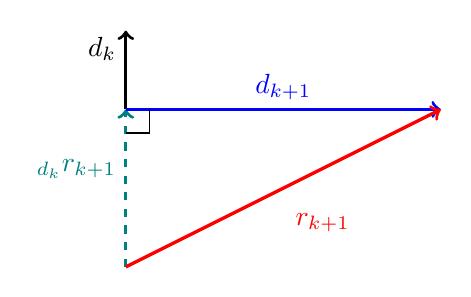
\begin{tikzpicture}
      % d_k dashed
      \draw[->, very thick, teal, dashed] (0, 0) -- (0, 2);
      % d_k
      \draw[->, very thick, black] (0, 2) -- (0, 3);

      % d_{k+1}
      \draw[->, very thick, blue] (0, 2) -- (4, 2);

      % r_{k+1}
      \draw[->, very thick, red] (0,0) -- (4, 2);

      % Right angle symbol
      \draw (0, 1.7) -- (0.3, 1.7) -- (0.3, 2);

      % Labels
      \node[above left, black] at (0, 2.5) {$d_k$};
      \node[above left, teal] at (0, 1) {$\pr_{d_k} r_{k+1}$};
      \node[above, blue] at (2, 2) {$d_{k+1}$};
      \node[below, red] at (2.5, 0.8) {$r_{k+1}$};
    \end{tikzpicture}

    \item В итоге алгоритм имеет следующий вид:

    \begin{equation*}
        \begin{dcases*}
            x_{k+1} = x_k + \alpha_k d_k\\
            r_{k+1} = r_k - \alpha_k A d_k\\
            \alpha_k = \frac{\langle d_k, r_k \rangle}{\langle d_k, r_k \rangle_A}\\
            d_{k+1} =  r_{k+1} - \frac{\langle r_{k+1}, d_k \rangle_A}{\langle d_k, d_k \rangle_A} d_k
        \end{dcases*}
    \end{equation*}
\end{itemize}

\subsubsection*{Свойства}

\begin{claim}
    Все векторы $r_k$ ортогональны между собой:

    \[
    \forall \, k_1 \neq k_2: \langle r_{k_1}, r_{k_2} \rangle = 0
    \]

    А также все $d_k$ $A$-ортогональны между собой:

    \[
    \forall \, k_1 \neq k_2: \langle d_{k_1}, d_{k_2} \rangle_A = 0
    \]
\end{claim}

\begin{proof}
    Будем доказывать по индукции по номеру итераций.

    \begin{itemize}
        \item База $k = 2$. Проверим, что $\langle r_1, r_2 \rangle = 0$ и $\langle d_1, d_2 \rangle_A = 0$.

        \[
        \langle r_1, r_2 \rangle = \left\langle r_1,
        r_1 - \frac{\langle d_1, r_1 \rangle}{\langle d_1, d_1 \rangle_A} A d_1
        \right\rangle =
        %
        \langle r_1, r_1 \rangle - \frac{\langle d_1, r_1 \rangle}{\langle d_1, d_1 \rangle_A} \langle r_1, A d_1 \rangle =
        %
        \langle r_1, r_1 \rangle - \frac{\langle r_1, r_1 \rangle}{\langle r_1, r_1 \rangle_A} \langle r_1, r_1 \rangle_A = 0
        \]

        $\langle d_1, d_2 \rangle_A = 0$ по определению.

        \item Предположение и шаг. Пусть вычислены $r_1, \ldots, r_k$ и $d_1, \ldots, d_k$ и выполнены условия ортогональности. Заметим, что

        \[
        \mathrm{span}(r_1, \ldots, r_k) = \mathrm{span}(d_1, \ldots, d_k),
        \]

        Можно доказать это равенство по индукции используя правила вычисления $r_{k+1}$ и $d_{k+1}$ в процессе алгоритма:

        \begin{equation*}
            \begin{aligned}
                &r_{k+1} = r_k - \alpha_k A d_k\\
                &d_{k+1} =  r_{k+1} - \frac{\langle r_{k+1}, d_k \rangle_A}{\langle d_k, d_k \rangle_A} d_k
           \end{aligned}
        \end{equation*}

        \begin{enumerate}
            \item Докажем ортогональность $r_k$. Вычислим $r_{k+1}$ по определению:

            \[
            r_{k+1} = r_k - \frac{\langle d_k, r_k \rangle}{\langle d_k, d_k \rangle_A} A d_k
            \]

            Поэтому вместо проверки $\langle r_{k+1}, r_i \rangle$ для $i \leqslant k$ можно проверить, что $\langle r_{k+1}, d_i \rangle$ для $i \leqslant k$. Эти утверждения равносильны. Случай $i = k$ проверяется построение. Для $i < k$:

            \[
            \langle r_{k+1}, d_i \rangle = \langle r_k, d_i \rangle - \frac{\langle d_k, r_k \rangle}{\langle d_k, d_k \rangle_A} \langle d_i, A d_i \rangle = 0 - 0 = 0 \text{ по предположению индукции}
            \]

            \item Докажем теперь $A$-ортогональность $d_k$. Случай $i = k$ проверяется построением. Для $i < k$:

            По определению $r_{i+1}$:

            \[
            r_{i+1} = r_i - \alpha_i A d_i \iff A d_i = \beta_i (r_{i+1} - r_i)
            \]

            По определению $d_{k+1}$:

            \[
            d_{k+1} = r_{k+1} - \pr_{d_k} r_{k+1} = r_{k+1} - \frac{\langle r_{k+1}, d_k \rangle_A}{\langle d_k, d_k \rangle_A} d_k
            \]

            Рассмотрим $ \langle d_i, d_{k+1} \rangle_A = \langle A d_i, d_{k+1} \rangle$:

            \begin{multline*}
                \langle A d_i, d_{k+1} \rangle = \beta_i \langle r_{i+1} - r_i, r_{k+1} \rangle - \beta_i \frac{\langle r_{k+1}, d_k \rangle_A}{\langle d_k, d_k \rangle_A} \langle r_{i+1} - r_i, d_k \rangle = \\ = \beta_i \langle r_{i+1} - r_i, r_{k+1} \rangle - \frac{\langle r_{k+1}, d_k \rangle_A}{\langle d_k, d_k \rangle_A} \langle A d_i, d_k \rangle = 0 - 0 \text{ по предположению индукции}
            \end{multline*}
        \end{enumerate}
    \end{itemize}
\end{proof}

\subsubsection*{Каноническая запись}

Найдем теперь $\langle d_k, r_k \rangle$, выразив $d_k$:

\[
\langle d_k, r_k \rangle = \langle r_k - \beta_k d_{k-1}, r_k \rangle = \langle r_k, r_k \rangle - \beta_k \langle r_k, d_{k-1} \rangle = \langle r_k, r_k \rangle - 0 = \langle r_k, r_k \rangle
\]

Так как линейные оболочки $\mathrm{span}(r_1, \ldots, r_k) = \mathrm{span}(d_1, \ldots, d_k)$ для всех $k$, то и $\langle r_k, d_{k-1} \rangle = 0$. Тогда получаем следующее:

\[
r_{k+1} = r_k - \frac{\langle r_k, r_k \rangle}{\langle d_k, d_k \rangle_A} A d_k
\]

Рассмотрим $\langle r_{k+1}, d_k \rangle_A = \langle r_{k+1}, A d_k \rangle$. Подставим $A d_k$ из выражения выше:

\[
\langle r_{k+1}, A d_k \rangle =
%
\left\langle
r_{k+1}, \frac{\langle d_k, d_k \rangle_A}{\langle r_k, r_k \rangle} \cdot (r_k - r_{k+1})
\right\rangle =
-\langle r_{k+1}, r_{k+1} \rangle \cdot  \frac{\langle d_k, d_k \rangle_A}{\langle r_k, r_k \rangle}
\]

Получаем, что

\[
d_{k+1} = r_{k+1} + \frac{\langle r_{k+1}, r_{k+1} \rangle}{\langle r_k, r_k \rangle} d_k
\]

Итоговый алгоритм на $k$-ой итерации:

\begin{equation*}
    \begin{dcases*}
        x_{k+1} = x_k + \alpha_k d_k\\
        r_{k+1} = r_k - \alpha_k A d_k\\
        \alpha_k = \frac{\langle r_k, r_k \rangle}{\langle d_k, r_k \rangle_A}\\
        \beta_k = \frac{\langle r_{k+1}, r_{k+1} \rangle}{\langle r_k, r_k \rangle}\\
        d_{k+1} = r_{k+1} + \beta_k d_k
    \end{dcases*}
\end{equation*}

\ProvidesFile{lecture-06.tex}[Лекция 6]

\newpage

\section{Метод бисопряженных градиентов}

\subsection*{Напоминание}

На прошлой лекции рассматривалась следующая задача:

$$
Ax = b,
$$

где $A_{n \times n}$ --- SPD матрица. Для таких матриц и был придуман метод сопряженных градиентов, который сходится за $n$ шагов в точной арифметике

\begin{itemize}
    \item Инициализация: $x_1 = 0$ (обязательно), $r_1 = b$, $d_1 = r_1$ --- вектор направлений

    \item $k$-ая итерация:

    \begin{equation*}
        \begin{dcases*}
            x_{k+1} = x_k + \alpha_k d_k\\
            r_{k+1} = r_k - \alpha_k A d_k\\
            \alpha_k = \frac{\langle d_k, r_k \rangle}{\langle d_k, d_k \rangle_A}\\
        \end{dcases*}
    \end{equation*}
\end{itemize}

Одной из главных особенностей метода сопряженных градиентов является ортогональность векторов невязок $r_k$ и направлений $d_k$ --- ключевое свойство для доказательства сходимости за $n$ шагов.
Можно ли построить такой же алгоритм для несимметричной матрицы $A$?

\subsection*{Двойственность}

\begin{definition}
    Пусть $V$ --- линейное пространство над полем $\mathbb{F}$. Тогда двойственным (или сопряженным) к нему пространством назовем:
    \[
        V^{\star} = \{f: V \longrightarrow \mathbb{F}: f \text{ --- линейное над } \mathbb{F} \}
    \]
\end{definition}

Скалярное произведение на линейном пространстве $V$ позволяет отождествить само пространство $V$ со множеством линейных функций на $V$:

\[
    f(x) = f \left( \sum\limits_i x_i e_i \right) = \sum\limits_i x_i f(e_i) = \sum\limits_i x_i f_i = \innerproduct{x}{f},
\]

то есть в ортонормированном базисе линейной функции со значениями $f_i$ на базисных векторах $e_i$ ставится в соответствие вектор $[f_1, \ldots, f_n]^{\top}$

Но если на пространстве $V$ не задано скалярное произведение, то и соответствия между $V$ и пространством его линейных функций можно построить, но будет зависеть от выбора базиса

По этой причине в методе бисопряженных градиентов строятся $4$ последовательности векторов: $2$ последовательности векторов и $2$ последовательности связанных с ними функций

\subsection*{Двойственность и линейные операторы}

Пусть $A: V \longrightarrow V$ --- линейный оператор, $f: V \longrightarrow \R$ --- линейная функция. Возьмем произвольный $x \in V$:

\[
    f^{\top} Ax = f(Ax) = \sum\limits_i f_i \sum\limits_j A_{ij} x_j = \sum\limits_j \left( \sum\limits_i A_{ij} f_i \right) x_j = (A^{\star} f)(x) = (A^{\top} f)^{\top} x
\]

То есть по $A$ мы можем построить линейный оператор $A^{\star}: V^{\star} \longrightarrow V^{\star}: A^{\star} = A^{\top}$


\subsection{Алгоритм}

\begin{itemize}
    \item Инициализация $x_1$. По начальному приближению строится вектор невязки $r_1 = b - Ax_1$.

    Затем задается линейная функция $\hat{r}_1 = \hat{r}_1(r_1) = \hat{r}_1^{\top} r_1 \neq 0$. Наиболее популярный вариант: $\hat{r}_1 = r_1$

    Векторы направлений строятся как $p_1 = r_1, \hat{p}_1 = \hat{r}_1$

    \item $k+1$-ая итерация:

    \begin{equation*}
        \begin{dcases*}
            x_{k+1} = x_k + \alpha_k p_k\\
            r_{k+1} = r_k - \alpha_k A p_k\\
            \hat{r}_{k+1} = \hat{r}_k - \alpha_k A^{\top} \hat{p}_k\\
            p_{k+1} = r_{k+1} + \beta_k p_k\\
            \hat{p}_{k+1} = \hat{r}_{k+1} + \beta_k \hat{p}_k\\
            \alpha_k = \frac{\hat{r}_k r_k}{ \hat{p}_k A p_k}\\
            \beta_k = \frac{\hat{r}_{k+1} r_{k+1}}{\hat{r}_k r_k}
        \end{dcases*}
    \end{equation*}
\end{itemize}

\subsection{Доказательство алгоритма}

\subsubsection*{Ортогональность}

\begin{claim}
    Для любых $i \neq j$ выполняются следующие условия:

    \[
        \begin{cases}
            \innerproduct{\hat{r}_i}{r_j} = \hat{r}_i^{\top} r_j = 0\\
            \innerproduct{\hat{p}_i}{Ap_j} = \hat{p}_i^{\top} A p_j = 0
        \end{cases}
    \]
\end{claim}

\begin{proof}
    Доказываем по индукции $k = \max(i, j)$

    \begin{itemize}
        \item Заметим, что (доказывается по индукции)
            \begin{align*}
                \mathrm{span}(r_1, \ldots, r_k) = \mathrm{span}(p_1, \ldots, p_k)\\
                \mathrm{span}(\hat{r}_1, \ldots, \hat{r}_k) = \mathrm{span}(\hat{p}_1, \ldots, \hat{p}_k)
            \end{align*}

        \item Пусть $j = k + 1, i < k$:
            \begin{align*}
                \hat{r}_i^{\top} r_{k + 1} &= \hat{r}_i^{\top} r_k - \alpha_k \hat{r}_i^{\top} A p_k = 0 - 0 = 0\\
                \hat{p}_i^{\top} A p_{k + 1} &= \hat{p}_i^{\top} \cdot \frac{r_k - r_{k + 1}}{\alpha_k} = \frac{1}{\alpha_k} \hat{p}_i^{\top} r_k - \frac{1}{\alpha_k} \hat{p}_i^{\top} r_{k + 1} = 0 - 0 = 0
            \end{align*}

        \item Для $i = k$ ортогональность выполняется из-за выбора коэффициентов $\alpha_k$ и $\beta_k$:
            \[
                \hat{r}_k^{\top} r_{k + 1} = \hat{r}_k^{\top} r_k - \alpha_k \hat{r}_k^{\top} A p_k = \hat{r}_k^{\top} r_k - \alpha_k \hat{p}_k^{\top} A p_k + \beta_{k - 1} \alpha_k \hat{p}_{k - 1} A p_k = 0\, (\text{подставим } \alpha_k)
            \]

            Аналогично для векторов направлений:

            \[
                \hat{p}_k A p_{k + 1} = (A^{\top} \hat{p}_k)^{\top} p_{k + 1} = (A^{\top} \hat{p}_k)^{\top} r_{k + 1} + \beta_k (A^{\top} \hat{p}_k)^{\top} p_k = -\frac{1}{\alpha_k} \hat{r}_{k + 1}^{\top} r_{k + 1} + \beta_k (A^{\top} \hat{p}_k)^{\top} p_k = 0
            \]
    \end{itemize}
\end{proof}


\subsection{Проблемы алгоритма}

\ProvidesFile{lecture-07.tex}[Лекция 7]

\newpage

\section{Предобуславливание}

\ProvidesFile{lecture-08.tex}[Лекция 8]

\newpage

\section{Собственные векторы и собственные значения}

\begin{definition}
    \textit{Собственным вектором} $v$ матрицы $A_{n \times n}$ с соответствующим \textit{собственным значением} $\lambda$ называется вектор, для которого выполнено:

    \[
    A v = \lambda v
    \]
\end{definition}

\subsection*{Постановка задачи: SPD матрица}

Задача нахождения (всех или нескольких) собственных векторов и собственных значений часто возникает на практике, особенно случай, когда $A_n$ является SPD матрицей, который будет рассматриваться сейчас

Для SPD матрицы известно, что существует ортонормированный базис из собственных векторов $e_1, \ldots, e_n$ с собственными значениями $\lambda_1, \ldots, \lambda_n$, где $\lambda_i > 0$

\subsection{Степенной метод}

\subsubsection*{Описание метода}

Следующий метод позволяет найти собственный вектор и соответствующее наибольшее собственное значение матрицы $A$

\begin{itemize}
    \item Сгенерируем случайный вектор $v_0: v^{\top} v = 1$

    \item Посчитаем $x_1 = A v_0$ и отнормируем его

    \item Проделаем то же самое с вектором $v_0 = x_1$

    \item При достаточном количество итераций получим $v_0$ --- собственный вектор с наибольшим собственным значением:

    \[
    \lambda = \frac{v_1^{\top} v_0}{v_0^{\top} v_0}
    \]
\end{itemize}

\subsubsection*{Сходимость метода}

Введем $\lVert \cdot \rVert_{2}$ норму. Пусть у матрицы $A$ есть базис из ортонормированных собственных векторов $e_1, \ldots, e_n$ и соответствующими собственными значениями $\lambda_1 > \lambda_2 \geqslant \ldots \geqslant \lambda_n$. Пусть $v_{0} = \sum x_i e_i$ --- некоторый вектор единичной длины с $x_1 \neq 1$. Определим последовательность

\[
v_{k+1} = \frac{A v_{k}}{\lVert A v_{k} \rVert}
\]



\[
\lVert A v_{k} \rVert \cdot v_{k+1} = A v_{k} = A^k v_0 =
%
\sum\limits_{i = 1}^n x_i A^k e_i =
%
\sum\limits_{i = 1}^n x_i \lambda_i^k e_i =
%
\lambda_1^k \left(
                x_1 e_1 + \sum\limits_{i = 2}^n x_i \cdot \left(\frac{\lambda_i}{\lambda_1}\right)^k e_i
            \right)
\]

Вспомним, что $\lambda_i / \lambda_1 < 1$, поэтому при достаточно больших $k$:

\[
\lVert A v_{k} \rVert \cdot v_{k+1} = A v_{k} =  \lambda_1^k (x_1 e_1 + \varepsilon_{k}),
\]

где $\lVert \varepsilon_{k} \rVert \longrightarrow 0$. Рассмотрим при $k \longrightarrow \infty$

\[
\lVert v_{k+1} - e_1 \rVert=
%
\left\lVert \frac{A v_{k}}{\lVert A v_{k} \rVert} - e_1 \right\rVert =
%
\frac{1}{ \lVert A v_{k} \rVert } \cdot \left\lVert \lambda_1^k (x_1 e_1 + \varepsilon_{k}) - \lVert A v_{k} \rVert \cdot e_1 \right\rVert \leqslant
%
\frac{1}{ \lVert A v_{k} \rVert } \cdot \Big| \lambda_1^k x_1 -  \lVert A v_{k} \rVert \Big| \cdot \lVert e_1 \rVert \longrightarrow 0
\]

Теперь последовательность:

\[
r_{k+1} =
\frac{
    \langle v_{k+1}, v_{k} \rangle
}{
    \langle v_{k}, v_{k} \rangle
} =
%
\frac{
    v_{k}^{\top} A v_k
}{
    v_k^{\top} v_k
} \longrightarrow
%
\lambda \cdot \frac{
    v_{k}^{\top} v_k
}{
    v_k^{\top} v_k
} = \lambda
\]

\subsubsection*{Как искать остальные?}

Зафиксируем сколь угодно малое $\varepsilon > 0$. Пусть мы нашли собственный вектор $v_1$ с наибольшим собственным значением $\lambda_1$. Построим матрицу $B = A - (\lambda_1 - \varepsilon) v_1 v_1^{\top}$. Так как $A$ является SPD матрицей, то

\[
A = U D U^{\top},
\]

где $U$ --- ортогональная матрица, столбцы которой являются ортонормированными собственными векторами, $D$ --- диагональная матрица из собственных значений $\lambda_i > \varepsilon$. Поэтому $A = \sum \lambda_i v_i v_i^{\top}$. Тогда

\[
B = A - (\lambda_1 - \varepsilon) v_1 v_1^{\top} = \varepsilon v_1 v_1^{\top} + \sum\limits_{i = 2}^n \lambda_i v_i v_i^{\top}
\]

Тогда если применить степенной метод для матрицы $B$, то мы можем получить собственный вектор со следующим по величине собственным значением

\paragraph{Замечание} Чтобы найти наименьшее собственное значение и соответствующий собственный вектор, то можем применить алгоритм к матрице $A^{-1}$. Чтобы вычислить $A^{-1} v_k$, мы можем вместо поиска $A^{-1}$, решать СЛУ $Az_k = v_k \iff z_k = A^{-1} v_k$

\subsubsection*{Поиск конкретного собственного значения}

Пусть у матрицы $A$ есть собственные значения $\lambda_1, \ldots, \lambda_n$ и мы хотим найти $\lambda_i$. Пусть мы знаем некоторое приближение $\lambda_i^{\star}$. Определим тогда матрицу $B = A - \lambda_i^{\star} I$ и рассмотрим ее спектр

\[
\spec(B) = \left\{ \lambda_k - \lambda_i^{\star} \right\} \implies \spec(B^{-1}) = \left\{ \frac{1}{\lambda_k - \lambda_i^{\star}} \right\}
\]

Получается, что если мы подобрали хорошее начальное приближение $\lambda_i^{\star}$, то $1 / (\lambda_i - \lambda_i^{\star})$ --- будем наибольшим собственным значением матрицы $B^{-1}$, которое мы можем найти с помощью степенного метода

\subsection{QR-разложение}

Следующий метод позволяет найти сразу несколько $m$ наибольших собственных значений и собственных векторов

Введем $\lVert \cdot \rVert_{2}$ норму. В этом методе нам понадобится процесс \href{https://en.wikipedia.org/wiki/Gram%E2%80%93Schmidt_process}{ортогонализации Грамма-Шмидта}. Пусть у нас есть векторы $v_1, \ldots, v_n$ и мы хотим получить ортонормированный базис $e_1, \ldots e_n$. Процесс описывается следующим образом:

\begin{itemize}
    \item Пусть $u_1 = v_1$. Теперь будем вычислять векторы $u_2, \ldots, u_n$ следующим образом:

    \[
    u_k = v_k - \sum\limits_{j = 1}^{k-1} \pr_{u_j} (v_k),
    \]

    где $\pr_{u_j} (v_k)$ --- проекция вектора $v_k$ на $u_j$

    \item Теперь $e_i = u_i / \lVert u_i \rVert$
\end{itemize}

\subsubsection*{Описание метода}

Пусть $V_{n \times m} = V_0 = (v_1 | \ldots v_m)$ --- матрица, чьи столбцы $v_i$ являются ортонормированными векторами. Тогда будем итеративно вычислять матрицу:

\[
V_{k+1} = \mathrm{ORT}(A V_k),
\]

где $\mathrm{ORT}$ --- процесс ортогонализации Грамма-Шмидта

При достаточно большом $k$ мы получим, что столбцы матрицы $V_k$ являются собственными векторами $e_1, \ldots, e_m$ с собственными значениями $\lambda_1 \geqslant \ldots \geqslant \lambda_m$

\subsubsection*{Сходимость метода}

Сходимость этого метода доказывается аналогично прошлому методу

\paragraph{Замечание} Аналогично прошлому методу мы можем найти первые $m$ наименьших собственных значений, применив метод к матрице $A^{-1}$


\end{document}
